\documentclass[11pt,a4paper]{article}
\usepackage[utf8]{inputenc}
\usepackage[german]{babel}
\usepackage[T1]{fontenc}
\usepackage{amsmath}
\usepackage{amsfonts}
\usepackage{amssymb}
\usepackage{graphicx}
\usepackage{colortbl}
\usepackage{color}
\usepackage[left=2cm,right=2cm,top=2cm,bottom=2cm]{geometry}
\author{Christian Weiß}
\title{Implementierung und Evaluirung eines SNMP Scanners}

\begin{document}
\renewcommand{\arraystretch}{1.2}
\definecolor{lgray}{gray}{.8}

% -----------------------------------------------------------------------------------------------------------------------------------------
% Definitionen
% -----------------------------------------------------------------------------------------------------------------------------------------
\newcommand{\emptyline}{\ \\}

% -----------------------------------------------------------------------------------------------------------------------------------------
% Titelblatt
% -----------------------------------------------------------------------------------------------------------------------------------------
\begin{figure}	% Logo
	\centering
	
\includegraphics[scale=.7]{Bilder/hsa.jpg}
	\label{img:logo}
\end{figure}
	
\vspace{\fill}

\begin{center}
	
	\begin{Huge}
		Abschlussarbeit\linebreak
	\end{Huge}
	
	\vspace{\fill}
	
	\begin{Large}
		Fakultät für Informatik\linebreak
	\end{Large}
	
	\vspace{\fill}
	
	\begin{LARGE}
		Titel\linebreak
	\end{LARGE}
	
	\vspace{1cm}
	
	\begin{Huge}
		\textbf{Implementierung und Evaluation eines SNMP Scanners}\linebreak
	\end{Huge}
	
	\vspace{\fill}
	
	\begin{Large}
		\begin{tabular}{r l}
			Autor: & Christian Weiß \\
			Prüfer: & Prof. Dr. Winter \\
			Datum: & \today \\
		\end{tabular}
	\end{Large}
	
\end{center}	% END - Titleseite
\pagebreak

% -----------------------------------------------------------------------------------------------------------------------------------------
% Inhaltsverzeichnis
% -----------------------------------------------------------------------------------------------------------------------------------------
\tableofcontents

% -----------------------------------------------------------------------------------------------------------------------------------------
% Einleitung (Motivation)
% -----------------------------------------------------------------------------------------------------------------------------------------
%\setcounter{page}{1}
\section{Einleitung}
Das Internet ist ein weltweiter Verbund von Rechnernetzwerken. Physikalisch besteht das Internet im Kernbereich aus einzelnen Netzwerken von Providern, Firmen und Universitäts- und Forschungsnetzwerke. Router verbinden diese Netzwerke miteinander.\\
Das Internet im Ganzen ist unbekannt. Selbst Netzbetreiber kennen nur einen kleinen Teil. Eine Verwaltung findet nur in den Subnetzen statt. Das macht eine Erfassung und Überwachung schwierig. Um den Zustand des Internet zu messen, sind viele Messstellen notwendig. Gut geeignet als Messstellen sind Endgeräte die sich regelmäßig Pakete durchs Internet schicken. Dieser Datenverkehr aus den Messungen kann Aufschluss über das Internet geben. Dafür wurde in der Hochschule eine App namens „Glimpse“ entwickelt, die auf allen erdenklichen Endgeräten installiert werden kann.
Glimpse verfügt über verschiedene Messmethoden, wie z.B. ein Bandbreitentest. Die Endgeräte sollen aus den Subnetzen, in denen sie sich befinden, die Bandbreite des Netzwerks zum Internet messen. Doch das Ergebnis einer solchen Messung kann keinen direkten Aufschluss zur Bandbreite geben. Waren zum Zeitpunkt der Messung noch andere Verbindungen aktive, so kann der gemessene Wert von der Bandbreite des Netzwerks stark Abweichen. Um nun eine bessere Einschätzung machen zu können, müsste man wissen, wie viele Verbindungen während der Messung bestanden haben. Diese Information hält ein Router in seinen Statistiken.\\
Es gibt verschiedene Protokolle mit denen Administratoren ihre Geräte im Netzwerk verwalten können. Darunter fallen Netconf und SNMP (Simple Network Management Protocol). Das Simple Network Management Protocol ist bereits weit verbreitet. Auf vielen Geräten wie Routern, Switches und Druckern ist vom Hersteller die Software bereits installiert. Ausgeliefert werden sie mit Standardpasswörtern, die von den Administratoren oft nicht geändert werden. Das bietet mir die Möglichkeit diese Geräte zu finden und auszulesen.
Findet sich im Subnetz von einem Glimpse-Client ein Gateway-Router, der mit den Standardpasswörtern läuft, können die Statistiken ausgelesen werden.
\pagebreak

% -----------------------------------------------------------------------------------------------------------------------------------------
% Geschichte
% -----------------------------------------------------------------------------------------------------------------------------------------
\section{Geschichte}
„Die Geschichte des SNMP hängt stark mit der Geschichte des Internets zusammen.[…]
So entstand im Jahre 1987 das SGMP (Simple Gateway Monitoring Protocol), da zu damaliger Zeit das Verbinden der Gateways das Hauptproblem war. Gleichzeitig entstand noch ein anderes Protokoll mit dem Namen HEMS (High Level Management Entity System), dessen Entwicklung schon länger zurückreichte. Allerdings fand dieses keine breite Unterstützung im Gegensatz zu dem SGMP, das schon zu dieser Zeit anfing, sich durchzusetzen. Ein weiterer Ansatz lag in einem OSI basierten Protokoll CMIP (Common Management Information Protocol) das auf TCP Protokoll aufgesetzt werden sollte und somit den Namen CMOT erhielt (CMIP over TCP). Aufgrund der geringen Durchsetzung von HEMS wurden nur SGMP und CMOT weiterentwickelt, ersteres, weil es schon weit verbreitet war und zweiteres, weil es auf einem langen ISO-standardisierten Untergrund aufbaute. Später sollten beide zu einem Protokoll verschmelzen.
1988 brachten die Entwickler um SGMP das RFC 1065 Structure of Managment Information [MR88b], RFC 1066 Managment Information Base [MR88a] und RFC 1067 Simple Network Managment Protocol [CFSD88] heraus, was dann 1989 zu recommended erklärt wurde, welches einem quasi-Standard entspricht und ab hier auch schon den Namen SNMP trägt. […]
SNMPv2 war allerdings von seinem Sicherheitsstandard her zu komplex, so dass dies keine breite Zustimmung fand und so wurde 1996 SNMPv2 nur mit dem Sicherheitsmanagement aus SNMPv1 noch mal als RFC eingereicht, was dann SNMPv2c genannt wurde. Doch auch diese Lösung wurde nicht als zufriedenstellend empfunden und so entstanden die beiden Standards SNMPv2u und SNMPv2*, die das Sicherheitsproblem lösen sollten.
Als letztes ist noch SNMPv3, RFC 2272-2275, zu erwähnen, das als Nachfolger von SNMPv2 zu verstehen ist, aber zusätzlich noch die Vereinigung von SNMPv2u und SNMPv2* bewirken soll [Bla97]. Diese wurde 1998 zum Proposed Internet Standard und dann 1999 zum Draft Internet Standard.“
\cite{history}
\pagebreak

% -----------------------------------------------------------------------------------------------------------------------------------------
% Netzwer Management
% -----------------------------------------------------------------------------------------------------------------------------------------
\section{Netzwerk Management}
„Netzwerkmanagement beinhaltet die Installation, Integration und Koordination von Hardware, Software und menschlichen Elemente zum Überwachen, Testen, Abfragen, Konfigurieren, Analysieren, Bewerten und Kontrollieren des Netzwerks und seiner Element-Ressourcen, um die Anforderungen in Bezug auf Performance im Betrieb und Dienstqualität zu angemessenen Kosten zu erfüllen.“
\cite{netmanagement}
\\
Netzwerkmanagement bedeutet, alle managebaren Entitäten zu Verwalten und Überwachen. Bei den Entitäten handelt es sich im wesentlichen um Router, Switches, Drucker und Server. Um diese Geräte veralten zu können muss sich ein Management System Informationen über den Status dieser Geräte im Netzwerk beschaffen können. Damit lassen sich die Information, die übers Netzwerk ausgetauscht werden, in zwei Kategorien einteilen. Es werden Nachrichten versandt, die über den Status einer Resource informieren und das Management System muss Kommandos an die Ressourcen senden können. Die Nachrichten über den Status können vom Management System angefordert sein, können aber auch vom Gerät selbst als Warnung bei einer Fehlfunktion verschickt werden. Das Management System kann mit Kommandos an Entitäten reagieren um einer Fehlfunktion entgegen zu wirken.
Die folgende Abbildung zeigt eine allgemeine Darstellung einer Netzwerkmanagementarchitektur mit ihren Hauptkomponenten. Die verwaltende Einheit als Rechner oder Notebook (NMS) und verwaltete Geräte mit ihren Agenten (A).
\\
\begin{figure}[h]
	\centering
	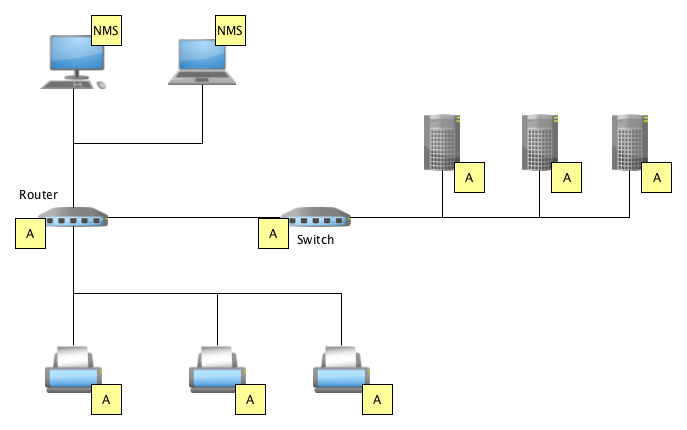
\includegraphics[scale=.5]{Bilder/Netzwerk.png}
	\caption{Beispiel Netzwerk mit allen Entitäten.}
\end{figure}

% -----------------------------------------------------------------------------------------------------------------------------------------
% Netzwerk Management System
% -----------------------------------------------------------------------------------------------------------------------------------------
\section{Network Management Station}
Eine NMS ist ein Rechner der im selben Netzwerk angesiedelt ist wie die Agenten mit denen es kommuniziert. Auf diesem Rechner läuft eine Software, die dem Administrator das Überwachen und Konfigurieren seiner Geräte im Netzwerk erlaubt. Eine NMS kann auch automatisiert sein und auf Fehlermeldungen der Agenten reagieren.
\\

% -----------------------------------------------------------------------------------------------------------------------------------------
% Agent
% -----------------------------------------------------------------------------------------------------------------------------------------
\section{Agenten}
Ein Agent ist ein Softwaremodul, dass auf einem netzwerkfähigem Gerät installiert ist. Diese Software bildet die Schnittstelle zwischen dem Gerät und dem Managementsystem. Ein NMS kann einen Request an den Agenten senden um den Status einer Resource zu erfragen. Der Agent liest die angeforderten Informationen aus seinem Wirt aus. Diese Informationen packt der Agent in einen RequestResponse und antwortet damit dem NMS. Die Eigenschaften eines Gerätes, welches von einem Agenten verwaltet wird, können vom NMS auch verändert werden. Zu den Informationen, die der Agent überwacht und übermitteln kann, gehören Konfigurationsdaten, Statusinformationen und Statistikwerte.
Kritische Eigenschaften eines Gerätes können vom Agent permanent überwacht werden. Triftet ein Wert einer Überwachten Eigenschaft in einen kritischen Bereich ab, kann das der Agent registrieren. Er reagiert sofort und sendet eine Warnung an das NMS.
Jeder Agent hat dazu eine Management Information Base (MIB) in der die Werte spezifiziert sind, die er verwalten und überwachen kann. Die Einträge in der MIB verweisen auf die Managed Objects vom Gerät.
\\
\begin{figure}[h]
	\centering
	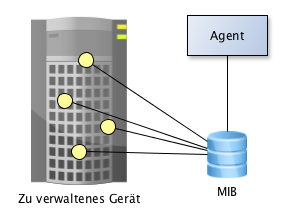
\includegraphics[scale=.7]{Bilder/Agent.png}
	\caption{EIn Agent und seine Managed Objects aus der MIB}
\end{figure}

% -----------------------------------------------------------------------------------------------------------------------------------------
% Agent
% -----------------------------------------------------------------------------------------------------------------------------------------
\section{Management Information Base (MIB)}
Die Management Information Base (MIB) enthält alle Managed Objects, die ein Agent später referenzierten kann. Die einzelnen Objekte müssen in der MIB detailliert beschrieben werden. Jedes Object erhält seine eigenen Zugriffsrechte, die später für die Anfragen von einem NMS an den Agenten gelten sollen. Damit durch ein NMS gezielt solche Objekte angesprochen werden können, erhalten die Managed Objects eine eindeutige Object ID (OID). Zudem sind zu bestimmen mit welchem Datentype der Status des Objekts anzugeben ist und es es gibt eine Beschreibung für das Objekt in Textform.\\
Die Module und Objekte einer MIB sind angeordnet in Baumform und können mit der OID referenziert werden. Ein Identifier zu einem Managed Object im Baum besteht aus Nummern und kann z.B. so aussehen: „.1.3.6.1.2.1.1“. Die Länge der OID bestimmt die Tiefe im Baum. Eine einzelne Nummer gibt Auskunft über das Blatt auf horizontaler Ebene. Die Blätter tragen auch Namen. So kann eine OID auch wie folgt beschrieben werden: „.iso.org.dod.mgmt.mib-2.system.sysDescr.0“.\\
Die Managed Objects einer MIB werden in der Syntax, die von der SMI vorgegeben wird, in einer ASCII-Datei abgelegt. Diese Datei kann von einem MIB-Compiler für die Verwendung durch einen Agenten aufbereitet werden.
\\
% toDo:
% ++++++++++++++++++++++++++++++++++++++++++++++++++++++++++++++++++++++++++++++
% Verschiedene Typen der Einträge : 		Scalar, Table, Spalte, Reihe
% (Netconf für SNMP Entwickler)
% ++++++++++++++++++++++++++++++++++++++++++++++++++++++++++++++++++++++++++++++
\begin{figure}[h]
	\centering
	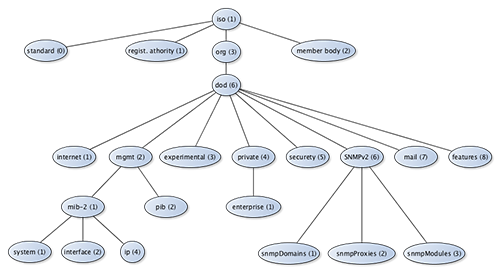
\includegraphics[scale=1]{Bilder/MIB.png}
	\caption{Die grobe Struktur des MIB-Baumes}
\end{figure}

% -----------------------------------------------------------------------------------------------------------------------------------------
% Structure of Management Information SMI
% -----------------------------------------------------------------------------------------------------------------------------------------
\section{Structure of Management Information (SMI)}
Die SMI ist eine Sprache zur Beschreibung der MIB’s und wurde für SNMP entwickelt. Damit lassen sich die Module, Managed Objects und Notifications für die MIB erstellen. Die SMI legt dazu die Syntax fest, mit der eine MIB beschrieben werden kann. Außerdem sind verschiedene Datentypen wie INTEGER, Gauge, Counter64 und viele mehr definiert. Die SMI ein für SNMP angepasster Auszug aus der ASN.1.
Ein Beispiel für einen MIB-Eintrag in der Form, wie sie von der SMI vorgegeben wird:
\\
\begin{figure}[h]
	\centering
	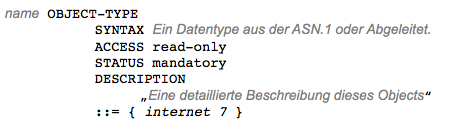
\includegraphics[scale=1]{Bilder/mibEintragSMI}
	\caption{Ein Eintrag in der MIB geschrieben mit den Vorgaben aus der SMI}
\end{figure}
Damit würde ein Eintrag im Baum entstehen, der  wie folgt zu erreichen ist: iso.org.dod.internet.neuesObj\\
und als Object Identifier : 1.3.6.1.7.0

% -----------------------------------------------------------------------------------------------------------------------------------------
% Abstract Syntax Notation One ASN.1
% -----------------------------------------------------------------------------------------------------------------------------------------
\section{Abstract Syntax Notation One (ASN.1)}
Zwischen den verschiedenen Geräten im Netzwerk kann es zu Inkompatibilitäten kommen. Die Hardware oder auch die installierte Software kann für die Daten unterschiedliche Darstellungen verwenden. Ein Beispiel dafür ware Big Endian und Little Endian. Bei der Kommunikation mit SNMP zwischen den Agenten und dem NMS müssen die Daten jedoch klar definiert sein. SNMP setzt für die Kompatibilität auf eine Teilmenge der ASN.1.\\
Die ASN.1 bietet einen Standard zur Definition von Datentypen und deren Werte. Ein Datentype ist eine Art von Information. Eine Information kann Beispielsweise eine Zahl, ein Text, ein Bilde oder auch ein Video sein. Für diese Informationen sollen Datentypen bereitgestellt werden. Ein Wert hingegen ist eine Instanz von einem dieser Datentypen. In der ASN.1 sind verschiede primitive Datentypen und deren Werte beschrieben. Außerdem finden sich Regeln um einfache Datentypen zu kombinieren, wodurch man komplexere Typen erzeugt. Es ist ein Werkzeugkasten um Daten in eine bestimmte  Form zu bringen.
\\

% -----------------------------------------------------------------------------------------------------------------------------------------
% Basic Encoding Rules BER
% -----------------------------------------------------------------------------------------------------------------------------------------
\section{Basic Encoding Rules (BER)}
Bei der Übertragung von Daten durch ein Netzwerk muss der Empfänger die Daten interpretieren können. Dafür ist immer ein Standard wie zum Beispiel ein Protokoll nötig. Die Basic Encoding Rules sind eines von drei Standards der ASN.1 zum Codieren der Daten. In dieser Codierung beschreiben und limitieren sich die Daten selbst. Die Daten werden mit einer Angabe über den Datentype und einer Angabe der die Länge in Bytes versehen. Gefolgt von den Daten selbst. Diese Vorgehensweise wird auch TLV-Encoding genannt. In einem eingehendem Datenstrom können Daten, die so codiert wurden, vom Empfänger leicht interpretiert werden. Der Empfänger muss noch nicht einmal die gesamte Nachricht erhalten, um einzelne Daten lesen zu können.
\\
\begin{figure}[h]
	\centering
	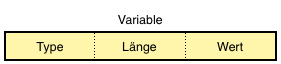
\includegraphics[scale=1]{Bilder/BasicEncodingRules}
	\caption{Darstellung eines Wertes in den Basic Encoding Rules}
\end{figure}

\subsection{Der Type}
Der Datentype wird normalerweise mit einem Byte bestimmt. Doch von diesem Byte sind die 3 höchsten Bit reserviert. So kann es vorkommen, dass der Datentype mit mehreren Bytes beschrieben wird. Mit fünf Bits können nur 31 verschiedene Typen definiert werden.
\\
\begin{figure}[h]
	\centering
	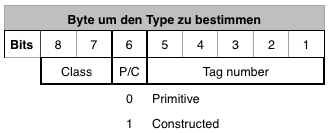
\includegraphics[scale=1]{Bilder/Datentype-BER}
	\caption{Die Verwendung der einzelnen Bits im Byte Datentype}
\end{figure}

Man unterscheidet zwischen komplexen und primitiven Datentypen. Primitive Typen sind einfache Datentypen wie zum Beispiel Integer. Komplexe Datentype sind Konstrukte bestehen aus mehreren einfachen Datentypen. Welcher Art das Datum ist, steht in Bit 6.
\\
Die Datentypen lassen sich außerdem in vier Klassen einteilen. Die Klassen sind Universal, Application, Context-specific und Private. Sie werden in den beiden höchsten Bits 7 und 8 dargestellt.
\\
\emptyline
\begin{tabular}{| l | c | c |}
	\hline
	\rowcolor{lgray}
	Klasse					&		Bit 8		& Bit 7\\
	\hline
	Universal				&			0		&	0\\
	\hline
	Application			&			0		&	1\\
	\hline
	Context-specific	&			1		&	0\\
	\hline
	Private					&			1		&	1\\
	\hline
\end{tabular}

\subsection{Die Länge}
Die Länge des Datums kann in drei verschiedenen Varianten auftreten. Sie kann in kurzer oder in langer Form angegeben werden. Beide sind definit. Die dritte Form is indefinit. Es wird keine Länge angegeben.

\subsubsection{Kurze definite Form}
Die einfachste Form, mit der die Länge eines Datums bestimmt wird, ist definit und ein Byte lang. Dazu muss in diesem Byte das höchste Bit 0 sein. In den restlichen 7 Bits kann die Länge des Datums in Bytes eingetragen werden. Dadurch, dass das höchste Bit 0 sein muss, liegt der Wertebereich nur bei 0 - 127 Bytes. Diese Notation ist also nur für Daten geeignet, die nicht länger als 127 Bytes sind.
\\
\begin{figure}[h]
	\centering
	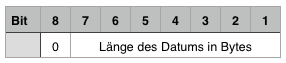
\includegraphics[scale=1]{Bilder/laengeDefinitKurz}
	\caption{Die Länge des Datums in kurzer definiter Form}
\end{figure}

\subsubsection{Lange definite Form}
Die lange definite Form der Längenangabe erstreckt sich über mehrere Bytes. So können sehr große Werte eingetragen werde. Dazu muss das erste Byte signalisieren, das sich die Längenangabe mehrere Bytes lang ist. Deshalb in diesem Byte das höchste Bit auf 1 gesetzt werden. Die Bits 7-1 geben auskunft über die Anzahl der Bytes, die folgen. Für einen 16 Bit Integer würden zum Beispiel zwei Bytes folgen. Eingetragen werden sie beginnen mit dem höchsten Byte.
\\
\begin{figure}[h]
	\centering
	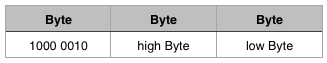
\includegraphics[scale=1]{Bilder/laengeDefinitLang}
	\caption{Die Länge des Datums in langer definiter Form}
\end{figure}

\subsubsection{Länge indefinit}
In der indefiniten Form wird keine Angabe über die Länge des Datums gemacht. Das Byte für die Längenangabe hat das höchste Bit auf eins gesetzt, was bedeuten würde, dass weitere Bytes für die Längenangabe folgen. Doch die Anzahl der folgenden Bytes wird mit 0 angegeben. Nun ist die Länge des Datums ungewiss. Die Bytes des Datums werden eingetragen. Da die Länge jedoch nicht bestimmt wurde, muss das Ende des Datums markiert werden. Eine "end-of-contents" Marke muss angehängt werden. Die "end-ofcontents" Marke besteht aus zwei leeren Bytes.
\\
\begin{figure}[h]
	\centering
	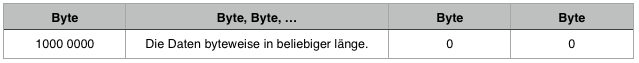
\includegraphics[scale=.75]{Bilder/laengeIndefinit}
	\caption{Die Länge in indefiniter Form}
\end{figure}

\subsection{Das Datum}
Das Datum selbst wird byteweise eingetragen, wobei mit dem höchsten Byte begonnen wird. Das niederste Byte komm zuletzt. Die Anzahl der Bytes muss mit der Längenangabe übereinstimmen.
\\

% -----------------------------------------------------------------------------------------------------------------------------------------
% Das SNMP Protokoll
% -----------------------------------------------------------------------------------------------------------------------------------------
\section{Das SNMP Protokoll}
SNMP steht für Simple Network Management Protocol. Es wurde entwickelt für die Kommunikation zwischen verschiedenen Geräten und einem NMS im Netzwerk.\\
\emptyline
Das mit diesem Protokoll angestrebte Ziel beschreiben die Entwickler wie folgt:\\
„The SNMP explicitly minimizes the number and complexity of management functions realized by the management agent itself.  This goal is attractive in at least four respects:\\
      (1)  The development cost for management agent software necessary to support the protocol is 	accordingly reduced.\\
      (2)  The degree of management function that is remotely supported is accordingly increased, 	thereby admitting fullest use of internet resources in the management task.\\
      (3)  The degree of management function that is remotely supported is accordingly increased, 	thereby imposing the fewest possible restrictions on the form and sophistication of 		management tools.\\
      (4)  Simplified sets of management functions are easily understood and used by developers of 	network management tools.\\
\emptyline
A second goal of the protocol is that the functional paradigm for monitoring and control be sufficiently extensible to accommodate additional, possibly unanticipated aspects of network operation and management.\\
\emptyline
A third goal is that the architecture be, as much as possible, independent of the architecture and mechanisms of particular hosts or particular gateways.“
\cite{rfcSnmpGoals}\\
\emptyline
Vom SNMP Protokoll gibt es heute mehrere Versionen. Die erste Version vom Protokoll hatte kaum Sicherheitsmechanismen. Im laufe der Zeit wurde es zu unsicher. Deshalb haben die Entwickler neue Entwürfe heraus gebracht. Die Version 2 von SNMP gibt es in mehreren Ausführungen mit verschiedenen Ansätzen zur Schliessung der Sicherheitslücken. Doch die Umsetzung der Versionen SNMPv2u und SNMPv2p waren den meisten Anwendern zu umständlich und fanden kaum Akzeptanz. Die Variante SNMPsec kam nie zu Einsatz und SNMPv2* wurde erst gar nicht veröffentlicht. Letztendlich verzichtete man auf die Sicherheitsmechanismen und brachte die Version SNMPv2c hervor. Damit wurde die erste Version mit den neuen Features der der zweiten Version erweitert. Um dem Verlangen nach Sicherheit doch noch gerächt zu werden, haben die Entwickler noch eine dritte Version aufgelegt, SNMPv3\\
Die Architektur besteht aus zwei einfachen Elementen, den Managern und den Agenten. Die Manager werden meist als Network Management Station (NMS) bezeichnet. Sie stellen Anfragen an die Agenten um Informationen über deren Gerät im Netzwerk zu erhalten. Sie können aber auch Änderungen an den Einstellungen eines Gerätes vornehmen. Das ermöglicht dem Administrator das zentrale Verwalten seiner Geräte im Netzwerk.\\
SNMP ermöglicht die Überwachung von Netzwerkkomponenten, bietet eine Fernkonfiguration und Fernsteuerung von Netzwerkkomponenten an. Außerdem gibt es eine Fehlererkennung mit Benachrichtigung. Agenten überwachen sich selbst, stellen sie dabei eine Fehlfunktion fest, senden sie eine Notifikation an ihre Management Station.\\
SNMP kann mit verschiedenen Transportprotokollen verwendet werden. Meistens werden die SNMP Pakete jedoch mit UDP versandt. Es können aber auch die Protokolle IPX, AppleTalk und OSI genutzt werde.\\
Mit SNMP werden Anfragen üder Status an ein Gerät im Netzwerk gestellt. Diese Anfragen (Request) können vom Gerät einen oder mehrere Werte als Antwort anfordern. Sie können das Gerät aber auch auffordern einen Wert in dessen Einstellungen zu ändern. Die Eigenschaften werden über ihren Object Identifier angesprochen und müssen in der MIB des Agents aufgeführt sein.\\
Wenn ein Request einen Fehler aufweist, also nicht dem Protokoll entspricht, dann ist vom Agent keine Antwort zu erwarten.\\
Zur Übertragung der Daten werden in allen Versionen die Basic Encoding Rules verwendet. Das gesamte Paket wird in dieser Form der Codierung geschrieben.
\\

% -----------------------------------------------------------------------------------------------------------------------------------------
% Protokolaufbau
% -----------------------------------------------------------------------------------------------------------------------------------------
\subsection{SNMPv1 Protokollaufbau}
\begin{figure}[h]
	\centering
	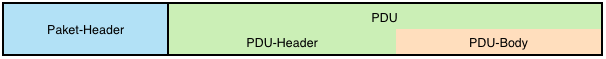
\includegraphics[scale=.8]{Bilder/SNMPv1-Aufbau.png}
	\caption{Der Protokollaufbau von SNMP Version 1}
\end{figure}
Das Paket unterteilt sich im im wesentlichen in zwei Teile. Der Header und die Protocol Data Unit (PDU). Der Header gibt Auskunft über die Länge des gesamten Pakets, die verwendete Protokoll Version und einen Community-Namen. In der PDU sind die zu übertragenden Daten enthalten, sowie eine Fehlermeldung.\\

\subsubsection{Header}
\begin{figure}[h]
	\centering
	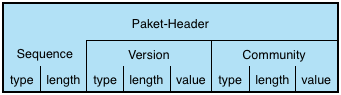
\includegraphics[scale=1]{Bilder/SNMPv1-Header.png}
	\caption{Der Header von SNMP Version 1}
\end{figure}
Der Inhalt eine SNMP Nachricht besteht aus einer Ansammlung von Daten, einer Sequenz. Der Header beginnt deshalb mit dem ASN.1 Datentype „Sequence“. Die Länge entspricht dem gesamten Paket in Bytes. Der rest des Paketes entspricht dem Wert in diesem TLV-Encoding.
Die Version die Version des Protokolls, die verwendet wird, ist vom Datentype INTEGER. Für die Länge ist hier nur ein Byte ausreichend. Die Versionsnummer sind fortlaufend durchnummeriert, beginnend bei 0 mit SNMPv1.\\
Die Community dient hier der Sicherheit und ist als eine Art Passwort gedacht. Es gibt ein solches „Passwort“ jeweils fürs Auslesen von Daten und zum Editieren von Konfigurationen an den Geräten. Vom Hersteller werden meist „public“ zum lesen und „private“ zum schreiben voreingestellt. Als Datentype verwendet man üblicherweise OCTED STRING. Für jedes Zeichen wird ein Byte verwendet.\\

\subsubsection{Protocol Data Unit (PDU)}
\begin{figure}[h]
	\centering
	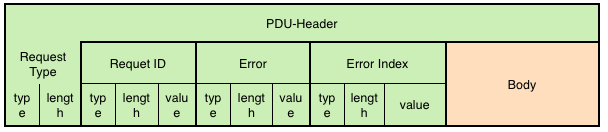
\includegraphics[scale=.8]{Bilder/SNMPv1-PDU.png}
	\caption{Die PDU von SNMP Version 1}
\end{figure}
Die PDU hat selbst auch einen Header. Im header wird der Request Type angegeben. Der Request Type ist vom Type IMPLICIT SEQUENCE. Die Typen geben den Zweck der Nachricht an. Zum Auslesen von Konfigurationsdaten sendet man „GetRequest“ oder „GetNextRequest“. Um die Konfiguration an einem Gerät zu ändern, sendet man einen „SetRequest“. Die Geräte antworten mit einem „RequestResponse“. Stellt ein Agent ungewöhnliche Werte an Gerät fest, sendet er eine „Trap“ Nachricht. Als Länge trägt man hier die gesamt Länge der PDU ein. Der rest der PDU entspricht dem Wert im TLV.\\
Außerdem enthält der Header eine Request ID, einen Fehlerwert und die Position des Fehlers. Jeder dieser Werte wird als TLV eingetragen.
Die Request ID ist ein beliebiger zahlen Wert, der die Nachricht eindeutig identifiziert.
Das Error-Feld kann einen von 0 verschiedenen Wert nur dann haben, wenn es sich um eine Antwort oder Benachrichtigung von einem Agent handelt. Mögliche Fehlermeldungen sind:\\
%\begin{figure}[h]
%	\centering
%	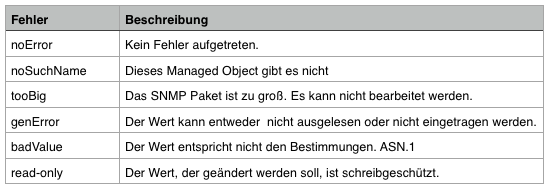
\includegraphics[scale=.75]{Bilder/SNMPv1-Fehler.png}
%\end{figure}
\emptyline
\begin{tabular}{| l | l |}
	\hline
	\rowcolor{lgray}
	Fehler				& Beschreibung\\
	\hline
	noError				& Kein Fehler aufgetreten.\\
	\hline
	noSuchName	&	Dieses Managed Object gibt es nicht.\\
	\hline
	tooBig				&	Das SNMP Paket ist zu groß. Es kann nicht bearbeitet werden.\\
	\hline
	genError			&	Der Wert kann entweder  nicht ausgelesen oder nicht eingetragen werden.\\
	\hline
	badValue			&	Der Wert entspricht nicht den Bestimmungen. ASN.1\\
	\hline
	read-only			&	Der Wert, der geändert werden soll, ist schreibgeschützt.\\
	\hline
\end{tabular}
\\
\emptyline
In einem SNMP Paket können mehrere Werte abgefragt werden. Dann enthält der PDU-Body mehrere Variablen Bindings. Wenn eine dieser Variablen einen Fehler verursacht, ist die Position dieser Variablen im Feld Error Index hinterlegt.\\

\subsubsection{PDU - Body}
\begin{figure}[h]
	\centering
	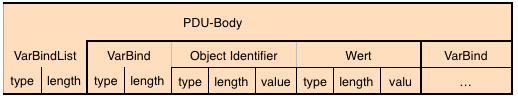
\includegraphics[scale=.8]{Bilder/SNMPv1-PDU-Body.png}
	\caption{Der Body aus der PDU. Der Teil mit den Variablen.}
\end{figure}
Im PDU-Body werden die Werte übertragen, die ausgelesen oder im Gerät gespeichert werden sollen. Die Variablen, es kann auch nur eine einzelne sein, werden in der "VarBindList" zusammen gefasst werden. Diese Liste der Variablen ist vom Type SEQUENCE. Auch hier wird alles TLV-Codiert, wie es in den BER definiert ist. Die einzelnen Variablen bestehen aus der OID des Managed Objects und dem zugehörigem Wert selbst. Die beiden werden ebenso überspannt von einer SEQUENCE, dem „VarBind“.\\
Der Object Identifier und der dazu gehörigeWert werden ebenfalls im TLV-Encoding eingetragen. Für eine Anfrage zum auslesen des Status einer Eigenschaft aus dem Gerät, soll kein Wert übermittelt werde. Den der Agent soll in seiner Antwort diesen Wert bereitstellen. In diesem Fall sendet man den Datentype NULL. Die Länge wird auch mit 0 angegeben und Daten im Feld ‚value‘ werden keine eingetragen.\\

\subsubsection{Veränderter Header bei Traps}
Ein Agent kann Teile des System auf dem er läuft selbstständig überwachen, so muss des Management System nicht permanent den Status abfragen. Der Agent kann konfiguriert werden auf bestimmte Werte ein Auge zu haben. Wenn eine dieser Systemeigenschaften eine kritische Marke über- oder unterschreitet, dann sendet der Agent eine Warnung an den Manager. Diese Art von Benachrichtigungen nennt man Traps. Für diese Traps gibt es einen eigenen PDU-Header.\\
\begin{figure}[h]
	\centering
	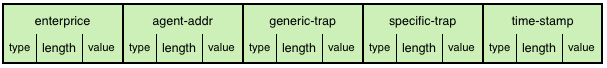
\includegraphics[scale=.8]{Bilder/SNMPv1-Header-Traps.png}
	\caption{Die Unterschiede im Header bei Traps}
\end{figure}
Gleich nach dem PDU Type folgt das Feld ‚enterprice‘. Im Feld ‚enterprise‘ ist immer ein Object Identifier zu finden. Er identifiziert die Eigenschaft, deren Wert für diese Warnung sorgte. Der Agent, der diese Nachricht versendet trägt seine IP-Adresse im Feld ‚agent-addr‘ ein. Der Datentype dafür ist festgelegt als NetworkAddress.\\
Das Feld ‚generic-trap‘ enthält einen Integer und kann folgende vordefinierte Fehler enthalten :\\
%\begin{figure}[h]
%	\centering
%	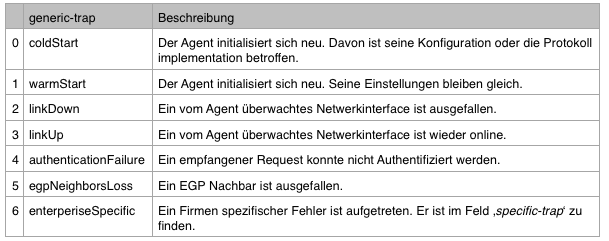
\includegraphics[scale=.8]{Bilder/SNMPv1-Traps-Fehler.png}
%\end{figure}
\begin{tabular}{| c | l | l |}
	\hline
	\rowcolor{lgray}
		& Fehler	&	Beschreibung\\
	\hline
	0	& coldStart						&	Der Agent initialisiert sich neu. Davon ist seine Konfiguration oder die\\
		&										&	Protokoll implementation betroffen.\\
	\hline
	1	& warmStart						&	Der Agent initialisiert sich neu. Seine Einstellungen bleiben gleich.\\
	\hline
	2	&	linkDOwn						&	Ein vom Agent überwachtes Netwerkinterface ist ausgefallen.\\
	\hline
	3	&	linkUp							&	Ein vom Agent überwachtes Netwerkinterface ist wieder online.\\
	\hline
	4	&	authenticationFalure	&	Ein empfangener Request konnte nicht Authentifiziert werden.\\
	\hline
	5	&	egpNeighborsLoss		&	Ein EGP Nachbar ist ausgefallen.\\
	\hline
	6	&	enterpriseSpecific			&	Ein Firmen spezifischer Fehler ist aufgetreten. Er ist im Feld ‚specific-trap‘\\
		&										&	zu finden.\\
	\hline
\end{tabular}
\emptyline

Das Feld ‚specific-trap‘ wird nur gebraucht, wenn der Fehler nicht einer der generischen Fehlertypen ist. Der Datentype ist als Integer festgelegt. Hier können vom Hersteller oder vom Administrator eigene Fehlertypen eingetragen werden.\\
Im letzten Feld übermittelt der Agent die Zeit, die seit seinem letzten Neustart vergangen ist. Der Zeitstempel wird angegeben mit dem Datentype TimeTicks.\\

% -----------------------------------------------------------------------------------------------------------------------------------------
% SNMPv2
% -----------------------------------------------------------------------------------------------------------------------------------------
\subsection{SNMPv2 Allgemein}
Es gibt mehrere Varianten von dieser SNMP Version. Die gängigste Varante aus der Version 2 des Protokolls is SNMPv2c Community Based. Ansonsten gab es noch SNMPsec, SNMPv2*, Party Based und User Based. „The Party-based SNMPv2 (SNMPv2p), SNMPv2u, and SNMPv2* were either declared Historic circa 1995 or were never on the standards track.“ \cite{rfcSnmpNotUsed}
\subsubsection{Sicherheit}
In der Version 2 des Protokolls ging es haupsächlich um die Sicherheit. Der Community-Name als eine Art Passwort ist zu unsicher geworden. Die Konfiguration der Geräte im Netzwerk sollte nicht länger dem Schutz eines solchen Passwortes unterliegen. Deshalb haben die Entwickler sich folgende Ziele gesetzt:
\begin{description}
	\item["(1)]
	The protocol should provide for verification that each received SNMPv2 message has not been modified during its transmission through the network 	in such a way that an unauthorized management operation might result.       
	\item[\ (2)]
	The protocol should provide for verification of the identity of the originator of each received SNMPv2 message.
	\item[\ (3)]
	The protocol should provide that the apparent time of generation for each received SNMPv2 message is recent.
	\item[\ (4)]
	The protocol should provide, when necessary, that the contents of each received SNMPv2 message are protected from disclosure.
\end{description}
In addition to the principal goal of supporting secure network management, the design of any SNMPv2 security protocol is also influenced by the following constraints:
\begin{description}
	\item[\ (1)]
	When the requirements of effective management in times of network stress are inconsistent with those of security, the former are preferred.
	\item[\ (2)]
	Neither the security protocol nor its underlying security mechanisms should depend upon the ready availability of other network services (e.g., 				Network Time Protocol (NTP) or secret/key management protocols).
	\item[\ (3)]
	A security mechanism should entail no changes to the basic SNMP network management philosophy."\ 
	\cite{rfcSnmpV2Securety}\\
\end{description}

\subsubsection{Authenzität und Vertraulichkeit}
Auf die Nachrichten wird ein Message Digest Algorithmus angewandt und das Ergebnis wird der Nachricht beigefügt. Zusätzlich kann eine Nachricht zum Versenden verschlüsselt werden. Dafür wird ein symmetrisches Verschlüsselungsverfahren benutzt. Beide verfahren zur Sicherheit sind optional, sie können angewandt werden, sind aber nicht verpflichtend.\\

\subsubsection{Features}
Außer den Sicherheitsvorkehrungen sind auch ein paar neue Features hinzugekommen. Dazu gehören folgende Nacrichtentypen und sonstige Erweiterungen:
\begin{itemize}
	\item 
		GetBulkRequest\\
		Dieser Request ermöglicht es dem Benutzer ganze Blocke aus der MIB zu lesen. Am nützlichsten ist GetBulk beim Auslesen von Tabellen. Wenn 				das Antwortpaket die maximale Größe überschreiten würde, dann sendet der Agent soviele Werte, wie er in einem Paket unterbringen kann. Ein 				GetRequest würde ein leeres Paket mit einer Fehlermeldung zurück liefern.
	\item
		Inform\\
		Wie ein auch bei einer Trap informiert der Agent mit einer Inform-Nachricht ein NMS über den Status des Gerätes. Eine Trap wird vom NMS 						angenommen und nicht quittiert.
	\item
		SNMPv2-Trap\\
		Die trap hat kein eigenes Nachrichtenformat mehr, wie in Version 1. Der PDU-Header von einer Trap ist der Gleiche wie von einem GetRequest.
	\item
		Erweiterungen in der SMI\\
		SMIv2 definiert neue Datentypen wie z.B. Counter64. Der MIB wurden Äste hinzugefügt wie z.B. mib-2 und snmpv2.
	\item
		Erweitertes Errorhandling\\
		Die Liste der Fehlermeldungen wurde erweitert.
\end{itemize}

% -----------------------------------------------------------------------------------------------------------------------------------------
% SNMPv2	Party Based
% -----------------------------------------------------------------------------------------------------------------------------------------
\section{SNMPv2 Party Based}
In diesem Modell von SNMP haben alle Agenten und Manager eine locale Datenbank, die Local Configuration Database (LCD). Die LCD ist eine Liste in der MIB mit den Parties eines Gerätes, die ein Agent oder Manager bei dieser Variante von SNMP haben muss. Die Parties sind alle Geräte, die der Agent bzw. der Manager kontaktieren darf. Sie legt außerdem fest welche Aktionen ein Agent bzw. Manager durchführen darf (Get, Set, Response, …). Weitere Information, die in der LCD enthalten sind, sind maximale Nachrichtenlänge, Verschlüsselungsverfahren, Athentitätsmechanismus, privates und öffentliches Passwort.\\
„Durch das sogenannte Party-Konzept wird eine Dreistufigkeit der Management-Hierarchie erreicht, da es nicht mehr nur Agenten und NMS gibt, sondern Node Manager, Lokale Manager und Super-Manager. Das führt für den Anwender wiederum dazu, dass er sich diese Hierarchie genauestens überlegen muss. SNMP2 hat drei verschiedene lokale Datenbanken, nämlich für unterstützte Parties, verwaltete Ressourcen und die Zugriffskontrollvorschriften. Die Formulierung von Zugriffsrechten und Gruppen ist relativ kryptisch. Durch die Notwendigkeit der Prüfung nach Zugehörigkeit zu bestimmten Gruppen, der Einordnung in einen bestimmten Kontext und des Geltungsbereichs der Rechte im Einzelnen ist eine SNMP2-Sendung bzw. ein SNMP2-Empfang zu einer komplexen zusammengesetzten Operation geworden. SNMP2 wurde bislang weder von Herstellern noch von Anwendern akzeptiert. Die Entwicklung wurde eingestellt.“
\cite{snmpv2PartyBased}\\

\subsection{SNMPv2p Protokollaufbau}
Der Aufbau des Protokolls unterscheidet sich grundlegend von der Vorgängerversion. Hier wurde sehr viel Wert auf Sicherheit gelegt. Der Absender trägt im Feld ‚privDest‘ einen Object Identifier ein und legt sich selbst als Empfänger einer Antwort fest. Durch den Object Identifier kann der Empfänger den Sender identifizieren. Das Paket wird nur bearbeitet, wenn der Absender bekannt ist. Den Rest des Pakets trägt man als OKTET STRING im Feld ‚privData‘ ein. Dieser Teil der Nachricht kann verschlüsselt sein. Wenn die Nachricht verschlüsselt wird, dann muss in der MIB des Empfängers der Schlüssel zum decodieren und das angewandte Verschlüsselungsverfahren eingetragen sein. Zu finden ist beides mit den Object Identifier aus Feld ‚privDist‘. Beide Felder werden eingebetet in eine Sequence, sie gibt die Länge der gesamten Nachricht an.\\
\begin{figure}[h]
	\centering
	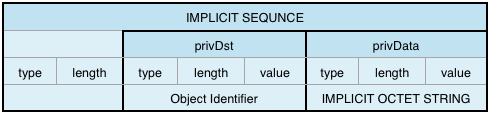
\includegraphics[scale=1]{Bilder/SNMPv2p-Header-Encode}
	\caption{SNMPv2 Party Based - Header zum Verschlüsseln der Nachricht.}
\end{figure}
Es folgt ein weiterer Header zur Sicherheit. Hier geht es um Authentizität. Es kann ein beliebiger Message Digest Algorithmus eingesetzt werden. Doch auch dieser muss in der MIB des Empfängers unter dem Object Identifier zu finden sein. Der Hashcode, den der Algorithmus erzeugt, wird im Feld ‚authInfo‘ eingetragen. Sollte auf Authentizität verzichtet werden, wird nur ein Octet String mit einer Länge von 0 Bytes eingetragen. Im Feld ‚authData‘ folgt die eigentliche Nachricht mit Header und PDU. Auf diesen Teil soll der Authentizitätsalgorithmus angewandt werden.\\
\begin{figure}[h]
	\centering
	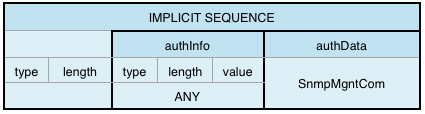
\includegraphics[scale=1]{Bilder/SNMPv2p-Header-Authentizitaet}
	\caption{SNMPv2 Party Based - Header für Authentizität.}
\end{figure}
Der eigentliche Header der Nachricht lässt sich mit dem aus der SNMP Version 1 nicht vergleichen. Gekapselt von einer Sequence trägt man hier Object Identifier ein. Das Feld ‚destParty‘ trägt den Object Identifier vom Empfänger dieser Nachricht. Der Absender, auch als Object Identifier, ist eingetragen im Feld ‚srcParty‘. Dann gibt es noch ein Feld ‚context‘, damit soll der Absender den Kontext der Nachricht angeben. Dieser Object Identifier spezifiziert einen Ast oder Teilbaum in dem die Werte zu finden sind, um die es sich in dieser Nachricht handelt. Die PDU bleibt im Vergleich zur Version 1 unverändert.\\
\begin{figure}[h]
	\centering
	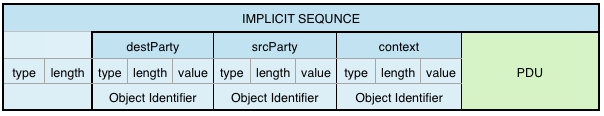
\includegraphics[scale=.8]{Bilder/SNMPv2p-Message}
	\caption{SNMPv2p Party Based - Die eigentliche Nachricht.}
\end{figure}

% -----------------------------------------------------------------------------------------------------------------------------------------
% SNMPv2	User Based
% -----------------------------------------------------------------------------------------------------------------------------------------
\section{SNMPv2 User Based}
\subsection{Datenbank mit User-Informationen}
Zur Sicherheitsstrategie der User Based Version gehört es, dass alle Benutzer, die auf Geräte zugreifen möchten, in einer Local Configuration Database (LCD) aufgeführt sind. Jedes Gerät hat eine LCD in seiner MIB.
Der Inhalt der LCD ist im wesentlichen :\\
\begin{itemize}
	\item{Benutzername (Octet String)}
	\item{Authentication Protocol (z.B. MD5)}
	\item{Privater Schlüssel des Benutzers für den Message Digest Algorithmus}
	\item{Verschlüsselungsprotokoll (symmetrische Verschlüsselung)}
	\item{Privater Schlüssel des Benutzers zur Verschlüsselung}
\end{itemize}
\textbf{Discovery}
„This security model requires that a discovery process obtain sufficient information about an SNMPv2 entity's agent in order to communicate with it.  Discovery requires the SNMPv2 manager to learn the agent's agentID value before communication may proceed. This may be accomplished by formulating a get-request communication with the qoS set to noAuth/noPriv, the userName set to "public", the agentID set to all zeros (binary), the contextSelector set to "", and the VarBindList left empty.  The response to this message will be an reportPDU that contains the agentID within the <parameters> field (and containing the usecStatsUnknownContexts counter in the VarBindList). If authenticated communication is required then the discovery process may invoke the procedure described in Section 2.7 to synchronize the clocks.“
\cite{rfcDiscoveryAgent}

\subsection{SNMPv2u Protokollaufbau}
Der Protokollaufbau von Version 2 user-based sieht dem, der Version 1 sehr ähnlich. Das Feld für Community im header wurde ersetzt durch ‚Parameter‘. Ein weiterer Unterschied zeigt sich im Bezug auf die PDU. Die PDU wird hier als Octet String eingetragen, nicht als Sequence wie es in den anderen Versionen üblich ist. Das hat den Vorteil, dass die PDU nun verschlüsselt werden kann. Bleibt die PDU umverschlüsselt, dann wird sie dem Nachrichten-Header als Sequence mit entsprechendem Type angehängt, wie es aus der Version 1 bekannt ist.\\
\begin{figure}[h]
	\centering
	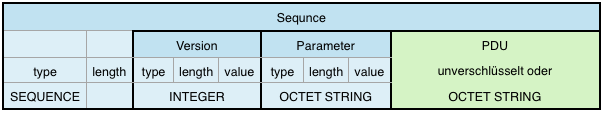
\includegraphics[scale=.8]{Bilder/SNMPv2u-Protokollaufbau}
	\caption{SNMPv2 User Based Protokollaufbau}
\end{figure}
\textbf{Parameter}\\
Das Feld 'parameter' soll als Octet String eingetragen werden. In diesem Octet String sollen allle Angaben aus der folgenden Tabelle enthalten sein.\\
\emptyline
\begin{tabular}{| l | c | l |}
	\hline
	\rowcolor{lgray}
	Parameter			& Octets	&		Beschreibung\\
	\hline
	model					&		1		&		Es gibt nur ein Model. Es kann aber ein anderes Model\\
								&				&		implementiert werden.\\
	\hline
	QoS						&		1		&		Zur Auswahl steht :\\
								&				&		\ - no authentication nor privacy\\
								&				&		\ - authentication, no privacy\\
								&				&		\ - authentication and privacy\\
								&				&		\ - generation of report PDU allowed\\
	\hline
	agentID				&		12	&		Ein Object Identifier, der den Absender identifiziert.\\
	\hline
	agentBoots			&		4		&		Eine vorzeichenlose Zahl, die angibt, wie oft der Agent\\
								&				&		gestartet wurde.\\
	\hline
	agentTime			&		4		&		Eine vorzeichenlose Zahl, die angibt, wie lange der Agent\\
								&				&		seit dem letzten Neustart \\
	\hline
	maxSize				&				&		Eine vorzeichenlose Zahl, die angibt, wie groß ein\\
								&				&		Antwortpaket sein darf.\\
	\hline
	userLength			&		1		&		Die länge des Usernamens. Max. 16 Octets.\\
	\hline
	userName				& x(1 - 16)&	Die einzelnen Zeichen des Usernamens. In der zuvor\\
								&				&		angegebenen Anzahl.\\
	\hline
	authLength			&		1		&		Die Länge des Wertes aus dem Message-Digest-Algorythmus.\\
	\hline
	authDigest			&x(0 - 255)&	Des Ergebnis vom Messge-Digest-Algorythmus, der auf die\\
								&				&		Nachricht angewandt wurde.\\
	\hline
	contextSelector	&x(0 - 40)&		Ein Ast oder Teilbaum in der MIB. Der Kontext um den es\\
								&				&		sich in der Nachricht dreht.\\
	\hline
\end{tabular}
\\
\emptyline

\textbf{Authentizität}\\
Für die Authentizität soll zunächst der Username in den Parametern eingetragen werden. Danach lässt man sich vom Massage Digest Algorithmus einen Hascode aus der ganzen Nachricht erzeugen. Anschließend ersetzt man den Username in den Parametern mit dem eben erzeugtem Hashcode.\\

% -----------------------------------------------------------------------------------------------------------------------------------------
% SNMPv2 Community
% -----------------------------------------------------------------------------------------------------------------------------------------
\section{SNMPv2 Community}
Nachdem die ersten Entwürfe von SNMPv2 zu umständlich und kompliziert waren, fanden sie keine Akzeptanz bei den Anwendern. Party Based und User Based SNMP kammen kaum zum Einsatz. Aus diesem Grund ging die Entwicklung wieder zurück zur Version 1. Für die Sicherheit hat man sich wieder auf einen Community-Namen als Passwort beschränkt. Damit ist SNMPv2c identisch mit der Verson 1. Der einzige Unterschied sind die Erweiterungen der Version 2 des Protokolls wie z.B. neue PDU Typen, kein Trap-Header und eine Erweiterte SMI.\\

% -----------------------------------------------------------------------------------------------------------------------------------------
% SNMPv3
% -----------------------------------------------------------------------------------------------------------------------------------------
\section{SNMPv3}
In der 3.Version von SNMP wurde nicht nur ein Protokoll beschrieben, sondern auch wie ein Agent oder NMS aufgebaut sein soll. Eine SNMP Entität bekommt eine Engine mit diversen Modulen. Sie enthält Applikationen zum Generieren von Nachrichten. Außerdem enthält die Engine ein Message Processing Subsystem, Security Subsystem und einen Dispatcher.
\subsection{Engine}
\begin{figure}[h]
	\centering
	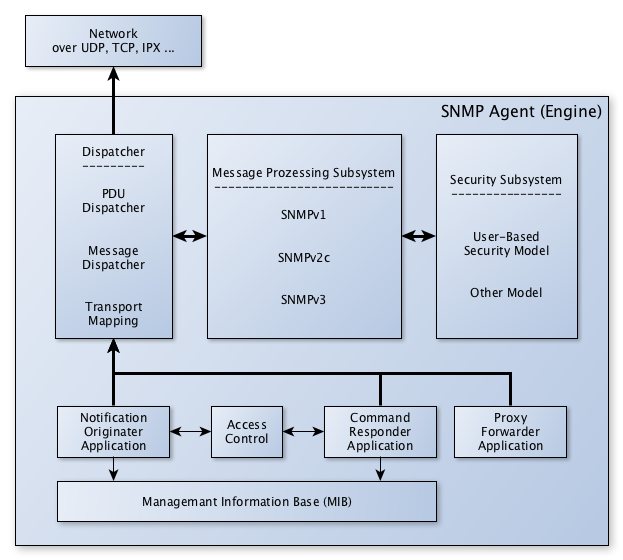
\includegraphics[scale=.6]{Bilder/SNMPv3-Engine-Agent.png}
	\caption{Die Engine eines SNMPv3 Agenten}
\end{figure}

\subsubsection{Dispatcher}
"There is only one Dispatcher in an SNMP engine.  It allows for concurrent support of multiple versions of SNMP messages in the SNMP engine. It does so by:
\begin{itemize}
	\item sending and receiving SNMP messages to/from the network,
	\item determining the version of an SNMP message and interacting with the corresponding Message Processing Model,
    \item providing an abstract interface to SNMP applications for delivery of a PDU to an application.
     \item providing an abstract interface for SNMP applications that allows them to send a PDU to a remote SNMP entity." \cite{rfcSnmpv3EngineDispatcher}
\end{itemize}

\subsubsection{Message Processing Subsystem}
"The Message Processing Subsystem is responsible for preparing messages for sending, and extracting data from received messages. Each Message Processing Model defines the format of a particular version of an SNMP message and coordinates the preparation and extraction of each such version-specific message format."
\cite{rfcSnmpv3EngineMPS}
„For incoming messages, a version-specific message processing module provides these values to the Dispatcher. For outgoing messages, an application provides these values to the Dispatcher.\\
For some version-specific processing, the values may be extracted from received messages; for other versions, the values may be determined by algorithm, or by an implementation-defined mechanism. The mechanism by which the value is determined is irrelevant to the Dispatcher.\\
The following additional or expanded definitions are for use within the Dispatcher.“
\cite{rfcSnmpEngineMPS2}

\subsubsection{Security Subsystem}
"The Security Subsystem provides security services such as the authentication and privacy of messages and potentially contains multiple Security Models."
\cite{rfcSnmpv3EngineSecurity}
Im Security Subsystem können mehrere Modelle implementiert sein. Als Standard ist das User-Based Security Model enthalten. Dieses Model bedient sich eines Keyed-Hash Message Authentication Code zur Gewährleistung der Authentizität und Integrität der übertragenen Daten.\\
Um auch für Vertraulichkeit zu sorgen, verwendet das User-Based Model einen Data Encryption Standard (DES) (in the cipher block chaining mode CBC) zur Verschlüsselung der Nachrichten. Die Verschlüsselung ist optional.\\
Im Protokoll-Header gibt es einen Abschnitt mit 'securityParameter'. Diese Paramerter sind abhängig vom Security Model und werden deshalb vom Security Subsystem eingetragen.
\begin{figure}[h]
	\centering
	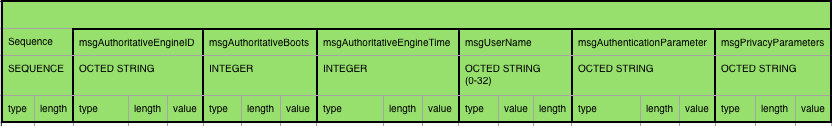
\includegraphics[scale=.58]{Bilder/SNMPv3-Header-SecParam.png}
	\caption{DIe 'Security Parameter' vom SNMPv3 Protokoll}
\end{figure}

\subsubsection{Access Control Subsystem}
"The Access Control Subsystem provides authorization services by means of one or more (*) Access Control Models. An Access Control Model defines a particular access decision function in order to support decisions regarding access rights."
\cite{rfcSnmpv3EngineACS} \\
Das Access Control Subsystem von einer SNMP Engine ist Verantwortlich für die Zugriffsberechtigungen auf die Managed Objects. Das Subsystem kann mehrere Modelle für Access Control habem. Der Standard ist das View-Based Access Control Model (VCAM). Die User können eingeschränkte Rechte auf bestimmte Instanzen von Objekten haben. die Zugriffsrechte werden in einer Local Configuration Database geklärt. Jedes SNMP Entity hat seine LCD in der MIB. In der LCD können durch einen Object Identifier, den Context-Namen, die Zugriffsrechte für eine Anfrage von einem Manager gelesen werden. In der LCD sind Einträge, Bereiche oder Teilbäume der MIB angegeben und mit den jeweiligen Zugriffsrechten versehen.\\
Die Zugriffsrechte auf Bereiche in der MIB:
\begin{itemize}
	\item Read-View
	\item Write-View
	\item Notify-View
\end{itemize}

\subsubsection{Applikationen}
Die Engine kann Verschiedene Applikationen enhalten:
\begin{itemize}
	\item Command Generator, zum Erstellen von Requests an den Agenten eines Gerätes im Netzwerk
	\item Command Responder, liest die vom NMS angeforderten Daten aus der MIB und generiert die Antwort.
	\item Notification Originator, erzeugt eine Benachrichtigung an das NMS bei kritischen Werten
	\item Notification Receiver, bearbeitet eingehende Notifikationen
	\item Proxy Forwarder, leitet Nachrichten weiter an eine andere Entität im Netzwerk
\end{itemize}

\subsection{SNMPv3 Protokollaufbau}
\subsubsection{Protokoll - Header}
\begin{figure}[h]
	\centering
	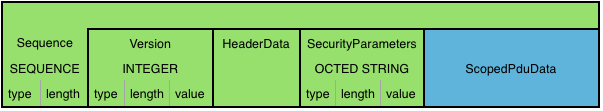
\includegraphics[scale=.8]{Bilder/SNMPv3-Header.png}
	\caption{Der Header des SNMPv3 Protokolls}
\end{figure}
Das Paket beginnt wie immer mit einer Sequence, die sich über die ganze Nachricht erstreckt und damit die Paketlänge angibt. Die Version muss hier mit 3 (SNMPv3) angegeben werden.\\
Im Feld ‚HeaderData‘ ist eine Sequence eingebetet, die ich nachfolgen separat beschreibe.\\
Die Security-Parameter werden an das ausgewählte Security-Model in der Engine übergeben. Die werte in diesem Feld sind abhängig von der Implementierung des Security-Models.
\begin{figure}[h]
	\centering
	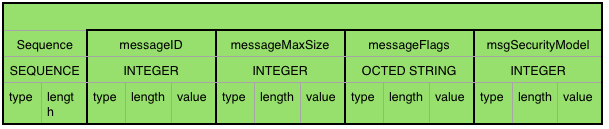
\includegraphics[scale=.8]{Bilder/SNMPv3-Header-Data}
	\caption{Der Ausschnitt 'HeaderData' aus dem Protokoll-Header}
\end{figure}
Jede Nachricht erhält eine ID, so können z.B. Requests und Responses einander zugeordnet werden. Dieses vorgehen ist bereits bekannt aus den Vorgängerversionen des Protokolls.
Der Sender gibt an, wie groß eine Antwort maximal sein darf, damit er sie bearbeiten kann.
Flags werden in einem Byte (OCTED) angegeben. Durch das Setzen der entsprechenden Bits, kann die verwendete Sicherheit angegeben werden. Zur Wahl stehen Authentifizierung und Verschlüsselung. Außerdem kann für bestimmte Fälle eine Antwort vom Empfänger erzwungen werden.\\
Als letzter Wert im Header wird ein, von der Engine des Empfängers unterstütztes, Security-Model gewählt.\\
\emptyline
Die Message Flags, mit denen bestimmt wird welche Sicherheitsmechanismen zum Einsatz kommen.
\begin{tabular}{| l | l |}
	\hline
	\rowcolor{lgray}
	messageFlag			&			Bit im Octed\\
	\hline
	authFlag					&			0000 0001\\
	\hline
	privFlag					&			0000 0010\\
	\hline
	reportableFlag			&			0000 0100\\
	\hline
\end{tabular}
\emptyline
Wenn eine Nachricht verschlüsselt ist, also das ‚privFlag‘ gesetzt wurde, dann muss auch eine Authentifizierung erfolgen. Das ‚privFlag‘ darf nicht ohne das ‚authFlag‘ gesetzt sein.

\subsubsection{Protocol Data Unit}
\begin{figure}[h]
	\centering
	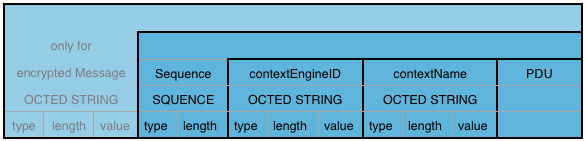
\includegraphics[scale=.8]{Bilder/SNMPv3-PDU.png}
	\caption{Die Protocol Data Unit im SNMPv3 Protokoll}
\end{figure}
Dieses Feld kann verschlüsselt oder unverschlossen übertragen werden. Ist das ‚privFlag‘ gesetzt, dann muss dieses Feld verschlüsselt werden. Es wird dann von einem OCTED STRING gekapselt, in dem byteweise der verschlüsselte Inhalt eingetragen wird.
Ansonsten wird der Octed String weggelassen und die PDU beginnt mit einer Sequence.\\
Die Engine ID wird angegeben in Verbindung mit dem PDU Type. Dadurch kann die Applikation der Engine bestimmt werden, welche die PDU bearbeiten soll.\\
Der Context-Name in Verbindung mit der Engine ID soll Aufschluss geben über die Managed Informations, die durch die PDU angefragt werden. Ein Context-Name kann in der LCD eines SNMP Entity’s nachgeschlagen werden, um die Zugriffsrechte zu ermitteln.
Die PDU selbst unterscheidet sich nicht von der in SNMP Version 1.\\

% -----------------------------------------------------------------------------------------------------------------------------------------
% Measurement
% -----------------------------------------------------------------------------------------------------------------------------------------
\section{SNMP Scanner}
\subsection{Vorgehensweise}
Die beste Methode alle SNMP-fähigen Geräte zu finden, wäre ein Portscan. Um in einem Subnetz nach Geräten zu suchen, die den Port 161 offen haben, müsste man ICMP-Nachrichten verschicken. Am besten such man zunächst nach allen Geräten im Netzwerk und sendet anschließend an jedes Gerät ein UPD Paket auf Port 161. Aus den ICMP Antworten kann sehr genau abgeleitet werden, an welcher Adresse ein SNMP Agent sitzt. Ein SNMP Agent würde eine Nachricht nur beantworten, wenn es ein korrektes SNMP Paket ist. Zum versenden von ICMP-Nachrichten sind administrative Rechte nötig. Die Anwendung verfügt jedoch nur über normale Benutzerrechte. Aus diesem Grund versendet der Scanner SNMP-Nachrichten und sammelt die Antworten.\\
Einige Versionen des Protokolls haben Sicherheitsmechanismen, die mir das Aufspüren dieser Geräte unmöglich machen. Ohne die Sicherheitsmechanismen zu hintergehen, kann ich nur Gräte finden, die mit den Versionen 1 und 2 Community-Based arbeiten.\\
Der Scanner kann auf zwei verschiedene Arten eingesetzt werden. Es kann ein automatischer Scan ausgelöst werden. Oder er kann vom Benutzer über die graphische Oberfläche gestartet werden.\\
Für den Scanner wird als Basisklasse ein QUdpSocket verwendet. Sehr viele SNMP Agenten arbeiten mit der Version 2c. Um dem Protokoll gerecht zu werden, reicht ein UDP Paket an dem Agent.\\

\subsection{Der automatische Scan}
Der Scanner muss zunächst konfiguriert werden. Er benötigt eine Liste an Community Namen und die zu verwendende Version des Protokolls, die im Paket an den Agent eingetragen werden. Weil UDP kein zuverlässiges Protokoll ist, kann außerdem ausgewählt werden, wie oft ein Paket an den Empfänger gesendet werden soll. Diese Werte zur Konfiguration kommen von einem Server und werden vor dem Start des Scanners von der ‚prepare()‘ Methode gesetzt.\\
Die zu durchsuchenden Subnetze kann der Scanner selbstständig finden. Es werden alle Netzwerkadapter geprüft, ob sie online sind und eine IPv4 Adresse verwenden. Alle Adapter, für die diese Bedingungen zutreffen, werden in einer Liste abgelegt.\\
\begin{figure}[h]
	\centering
	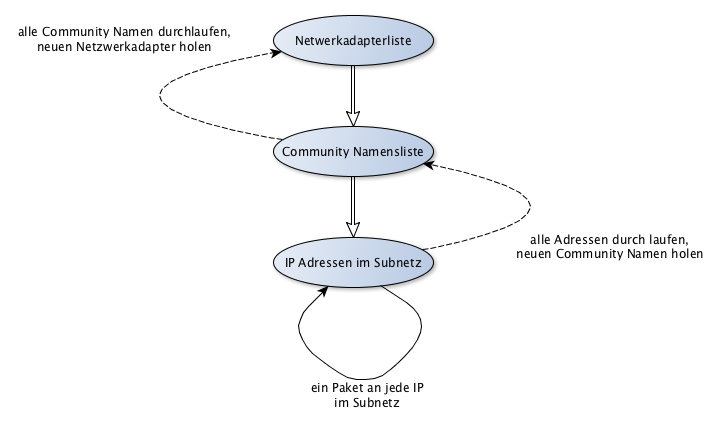
\includegraphics[scale=.6]{Bilder/SchemaScanner.png}
	\caption{Das grobe Ablaufschema des Scanners}
\end{figure}
Die Abbildung zeigt den Ablauf beim suchen nach Geräten im Subnetz. Von jedem Adapter, der online ist, wird der IP Adressenbereich vom Subnetz errechnet. Mit jedem in der Liste enthaltenem Community-Namen wird wenigstens ein Datenpaket an jede IP Adresse gesendet.\\

\subsection{Netzwerkadapter und ihre Subnetze}
Um die Netzwerkinterfaces zu verwalten bietet Qt eine Klasse QNetworkInterface. Diese Klasse hat eine statische Methode, die alle Adapter ausgibt. Allerdings sind in der Liste auch Anschlüsse wie FireWire und Bluetooth enthalten. Diese Anschlüsse sowie Adapter die nicht mit einem Netzwerk verbunden sind, sollen aussortiert werden. Ausserdem beschränke ich die Auswahl auf IPv4 Adressen. Alle Interfaces mit einer IPv4 Adresse und einer Hardwareadresse (Mac) sollen vom Scanner verwendet werden.\\
Um das Subnetz zu erfassen, werden die Ip Adresse und die Netmask benötigt. Beides kann mit Hilfe der Klasse QNetworkInterface abgefragt werden.
Zu erst wird die kleinste Ip Adresse (Untergrenze) eines Subnetzes ermittelt. Durch eine bitweise Verknüpfung mit dem logischen UND, ergibt sich aus der Ip Adresse des Netzwerkinterfaces und der Netmask die Untergrenze.\\
Für die größte Ip Adresse des Subnetzes (Obergrenze) brauche ich das Negativ der Netmask. Verknüpfe ich nun die negative Netmask und die Untergrenze mit dem logischem ODER, so erhalte ich die Obergrenze.\\
In der Tabelle unten ist ein Beispiel angeführt. Für dieses Beispiel wurde die Ip Adresse „171.82.170.52“ und die Netmask „255.255.240.0“ verwendet.\\
\begin{figure}[h]
	\centering
	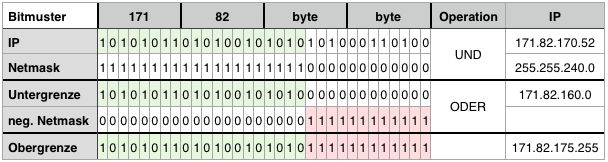
\includegraphics[scale=.8]{Bilder/IpRange.png}
	\caption{Die Ober- und Untergrenze eines Subnetzes ermitteln.}
\end{figure}
Die grüne Markierung zeigt, das durch die logischen Operationen der Vordere Teil der IP Adresse sich nicht verändert. Genau wie es die Netmask vorgibt.\\
Durch die rote Markierung wird demonstriert wie der hintere Teil der IP Adresse auf den höchsten Wert gesetzt wird.\\

\subsection{Scan starten}
Aus der Liste der Netzwerkadapter wird ein Adapter entnommen. Es wird die kleinste und die größte IP Adresse seines Subnetzes ermittelt. Danach wird der erste Community Name aus der Liste gewählt. Mit diesem Namen für die Community wird ein Paket für eine SNMP Anfrage an einen Agenten erzeugt. Das Paket wird an alle Adressen in der zuvor erhaltenen Reichweite des Subnetzes gesendet.\\

\subsection{Senden an alle Adressen in Subnetz}
Ein UDP Paket wird mit der Methode ‚writeDatagram()‘ aus der Klasse QUdpSocket versendet. Ist das erste Datenpaket fehlerfrei versandt, dann wird ein Timer gestartet. Der Timer löst in einem einstellbarem Interval ein Signal aus. Durch dieses Signal wird die Methode ‚timerEvent()‘ aufgerufen. Diese Methode inkriminiert die IP und sendet das nächste Paket an diese Adresse. Wenn die letzte IP-Adresse im Subnetz erreicht ist, dann wird der Timer gestoppt. An diesem Punkt sollte jeder Agent eine Anfrage erhalten haben. Doch um sicher zugehen, kann der Vorgang wiederholt werden und das gleiche Paket noch einmal an alle Adressen gesendet werden. Dazu wird das Signal ‚retry()‘ wird ausgelöst, wodurch die Methode ‚doRetry()‘ aufgerufen wird.\\
\begin{figure}[h]
	\centering
	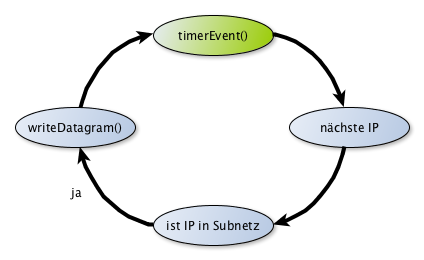
\includegraphics[scale=.6]{Bilder/InnererKreis.png}
	\caption{Der Ablauf beim Versenden einzelner Pakete.}
\end{figure}

\subsection{Retries}
Da UDP ein nicht zuverlässiges Protokoll ist, können Pakete im Netzwerk verloren gehen. Kommt von einer Adresse keine Antwort, ist nicht gewiss, dass dort kein Agent horcht. Aus diesem Grund müssen alle Adressen, von denen keine Antwort kam, noch einmal geprüft werden. Dazu kann die Anzahl der Versuche eingestellt werden, um einen Agent an einer IP mit einem Community Namen möglichst zuverlässig zu erreichen. Dafür wird der zuvor beschriebene Kreislauf mit der gewünschten Anzahl wiederholt. Bis alle Wiederholungen abgeschlossen sind, danach wird der Timer gestoppt und das Signal ‚changeSnmpCommunity()‘ ausgelöst. Daraufhin wird ein neues Datenpaket mit einem anderen Community Namen geschnürt.\\

\subsection{Warum Wiederholungen auf alle Adressen}
Um nicht erneut Pakete an alle Adressen zu senden gäbe es verschiedene Möglichkeiten. Es könnte zum Beispiel nach dem Senden eines Paketes auf eine Antwort gewartet werden. Um dann gleich nachdem keine kam das nächste Paket zu senden. Doch dafür wäre ein Timeout nötig. In einem einfachen kleinem Netzwerk sind meist 254 Adressen verfügbar. In so einem kleinen Netzwerk ist im Schnitt mit ca. fünf Treffern zu rechnen. Also müsste 249 malvergeblich auf eine Antwort gewartet werden. Beträgt der Timeout nur eine Sekunde, dann würde ein Scan für dieses Beispiel mit nur einem Community Namen mehr als 249 Sekunden dauern. Das sind gut vier Minuten und dauert damit viel zu lange.\\
Alternativ könnte man eine Liste führen. Eine Liste mit all den IP Adressen, von denen ein Agent geantwortet hat. Dann könnte man diese Adressen beim nächsten Durchlauf ausschließen. Jede Adresse müsste dann mit dem Ergebnis aus dem ersten Durchlauf abgeglichen werden, bevor ein Paket dorthin versendet wird. Doch um fünf Adressen aus 254 auszuschließen halte ich für einen zu großen Overhead.\\
Deshalb werden ohne vorherige Ergebnisse zu berücksichtigen erneut Pakete an alle Adressen gesendet. Die Selektion findet dann nach dem Scannen statt. Da die Ergebnismenge wesentlich kleiner ist als die Anzahl der Adressen in einem Subnetz, halte ich dieses Vorgehen für effektiver.\\

\subsection{Community Namen}
Auf vielen Geräten werden vom Hersteller bereits SNMP Agenten installiert. Mit der standard Konfiguration nutzen diese Agents die Community-Namen „public“ und „private“. Der Kunde kann diese jedoch beliebig ändern. Doch der Scanner sollte wenigstens die Gräte finden, die noch die standard Konfiguration verwenden. Dazu sollten wenigstens diese beiden Namen ausprobiert werden. Die Liste der Namen kann in der Konfiguration auf dem Server beliebig angelegt werden.\\
Ist ein Scan mit allen Wiederholungen abgeschlossen und das Signal ‚changeSnmpCommunity()‘ ausgelöst, dann holt eine Methode den nächsten Community-Namen aus der Liste. Mit dem Community-Namen muss ein neues SNMP Paket gebaut werden. Das neue Paket wird auf die erste Adresse im Subnetz mit der Methode ‚writeDatagram()‘ gesendet. Der Timer wird gestartet, wodurch der Kreislauf erneut angestoßen wird.
Wenn alle Community-Namen der Liste bereits verwendet wurden, wird das Signal ‚changeInterface()‘ ausgelöst.\\

\subsection{Netzwerkadapter wechseln}
Sind an einem Netzwerkadapter alle Community-Namen an allen Adressen mit sämtlichen Wiederholungen durch, wird ein anderer Adapter ausgewählt. Durch ein Signal wird die Methode ‚nextInterface()‘ aufgerufen, in der aus der Liste der Adapter der nächste heraus genommen wird. Für diesen Adapter wird der Adressraum bestimmt. Aus der Liste der Community-Namen wird der erste in der Liste gewählt. Mit diesem Namen wird ein neues Paket erzeugt. Das neue Paket wird mit der Methode ‚writeDatagram()‘ an die erste IP im Subnetz geschickt und der Timer gestartet. Damit beginnt der Zyklus in dem Subnetz dieses Adapters von neuem.\\
Ist kein Netzwerkadapter mehr in der Liste, ist das Scannen abgeschlossen. Es wird ein Timer mit einer Sekunde gestartet um auf ausstehende Antworten zu warten. Danach wird der Scanner beendet und das Signal ‚scanFinished()‘ ausgelöst. Diesem Signal wird ein Zeiger auf das Ergebnis des Scans mit gegeben. Ein Empfänger dieses Signals kann das Ergebnis auswerten.\\

\subsection{Fehlerbehandlung}
Für die Fehlerbehandlung gibt es eine Membervariable vom Type ‚QString‘. Sie enthält eine Beschreibung des aufgetretenen Fehlers.\\
\textbf{Beim Starten des Scanners}\\
Wenn ein automatischer Scan gestartet wird, dann wird nach Netzwerkadaptern gesucht, die mit einem Subnetz über Ipv4 verbunden sind. Kann der 	Scanner keinen Netzwerkadapter mit Verbindung finden, dann endet die Methode und gibt ‚false‘ zurück. Die Membervariable wird mit dem 						Fehlertext „No online network interface available.“ belegt.\\
\textbf{Beim Senden der UDP Pakete}\\
Die Klasse ‚QUDPSocket‘ löst ein Signal aus, wenn ein Fehler auftritt. Dieses Signal wird abgefangen. Die Fehlermeldung wird erzeugt und in der 				Membervariablen gespeichert. Da das Scannen asynchron läuft, wird der Intervaltimer gestoppt und das Signal ‚reportError(QString)‘ ausgelöst.

% -------------
\newpage
% -----------------------------------------------------------------------------------------------------------------------------------------
% Literaturverzeichnis
% -----------------------------------------------------------------------------------------------------------------------------------------
\begin{thebibliography}{10}
	\bibitem{history}			% Geschichte
	\begin{small}
		www-i4.informatik.rwth-aachen.de/content/teaching/proseminars/sub/2003\_ss\_proseminar\_docs/snmp.pdf
	\end{small}
	\bibitem{netmanagement}	% Netzwerk Management
		Kurose, J. F.,
		Computernetze: Ein Top-Down-Ansatz mit Schwerpunkt Internet,
		Addison-Wesley,
		2002
	\bibitem{rfcSnmpGoals}
		RFC 1157, Goals of the Architecture, Seite 5
	\bibitem{rfcSnmpNotUsed}
		RFC 3410, 8.2.  SNMPv1 and SNMPv2 Standardization Status, Seite 21, Absatz 1
	\bibitem{rfcSnmpV2Securety}
		RFC 1446, 1.3.  Goals and Constraints, Seite 5
	\bibitem{snmpv2PartyBased}
		http://www.comconsult-research.de/snmp-versionen-2-und-3/,
		ComConsult Research, Das Wissensportal, SNMP Version 2 und 3
	\bibitem{rfcDiscoveryAgent}
		RFC 1910, 4. Discovery, Seite 30
	\bibitem{rfcSnmpv3EngineDispatcher}
		RFC 3411,  3.1.1.2 Dispatcher, Seite 18
	\bibitem{rfcSnmpv3EngineMPS}
		Quelle: RFC 3411, 3.1.1.3, Message Processing Subsystem, Seite 19
	\bibitem{rfcSnmpv3EngineSecurity}
		RFC 3411, 3.1.1.4 Security Subsystem, Seite 20
	\bibitem{rfcSnmpv3EngineACS}
		RFC 3411, 3.1.2  Access Control Subsystem, Seite 21
	\bibitem{rfcSnmpv3EngineMPS2}
		RFC 3412, 3. Elements of Message Processing and Dispatching, Seite 6
\end{thebibliography}

\end{document}